\subsection{Machine Learning Approach}
Μια διαφορετική υλοποίηση που έχουμε να προτείνουμε είναι μια προσέγγιση με τεχνικές Μηχανικής μάθησης. Όπως αναφέρεται και στο \cite{mldef} η Μηχανική μάθηση είναι υποπεδίο της επιστήμης των υπολογιστών που αναπτύχθηκε από τη μελέτη της αναγνώρισης προτύπων και της  υπολογιστικής θεωρίας μάθησης στην τεχνητή νοημοσύνη. Πιο συγκεκριμένα κάνουμε χρήση επιβλεπόμενης μάθησης (supervised learning) κατά την οποία το υπολογιστικό πρόγραμμα δέχεται τις παραδειγματικές εισόδους καθώς και τα επιθυμητά αποτελέσματα από έναν «δάσκαλο», και ο στόχος είναι να μάθει έναν γενικό κανόνα προκειμένου να αντιστοιχίσει τις εισόδους με τα αποτελέσματα.
Πιο αναλυτικά:
\begin{itemize}
  \item \textbf{Παραδειγματικοί είσοδοι:} Αρχεία Wav των 8 KHz, 8 bit, mono των 8s εκτελεσμένα από διάφορους χρήστες από τη βάση MIR-QBSH-corpus. %TODO put link
  \item \textbf{Χαρακτηριστικά (features):} 14 Pitch Vectors μέσω της μεθόδου Cepstral\cite{cepstral} με μήκος παραθύρου 1s και μήκος επικάλυψης 0.5s. Ο λόγος είναι γιατί θεωρήσαμε ότι το ένα δευτερόλεπτο αρκεί για να περιγράψει επαρκώς ένα σημείο του τραγουδιού.
   %TODO put the plot that shows why we chose that
  \item \textbf{Επιθυμητά αποτελέσματα:} Τα labels των παραπάνω τραγουδιών, δηλαδή το όνομα του καθενός.
\end{itemize}

\begin{figure}
        \centering
        \vspace{-20pt}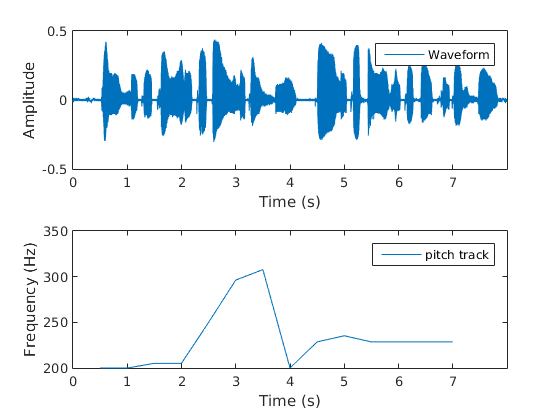
\includegraphics[height=7cm, width=\linewidth]{machine_learning/pitchvector_cepstrum}
        \vspace{-20pt}\caption{Pitch Vectors με παράθυρο 1000ms και επικάλυψη 50\%.}
        \label{fig:pvcepstrum}
\end{figure}

Σημαντικό είναι να πούμε ότι χρησιμοποιήσαμε μικρό πλήθος τραγουδιών και συγκεκριμένα 9 λόγω του μικρού μεγέθους των δειγμάτων που είχαμε και σε σχέση με αυτό των features που επιλέξαμε. Επίσης κάναμε τις εξής θεωρήσεις, οι οποίες προέκυψαν από τη βάση δεδομένων που χρησιμοποιήσαμε:
\begin{enumerate}
  \item Καθώς χρησιμοποιούμε παράθυρα των 1s με overlap 50\%, θεωρούμε ότι τα κομμάτια θα πρέπει να είναι εκτελεσμένα με καθυστέρηση το πολύ 500ms (π.χ. λόγω διαφορετικού tempo).
  \item Η εκτέλεση του κάθε τραγουδιού ξεκινάει πάντα από την αρχή.
\end{enumerate}
Στην αρχή χρησιμοποιήθηκαν μοντέλα μηχανικής εκμάθησης όπως: %TODO put the images here 
\begin{itemize}
  \item Δέντρα Απόφασης (Copmlex Trees) - Overall Accuracy 55.3\%  
  \item k-Nearest Neighbors Algorithm 	- Overall Accuracy 54.7\%
  \item Cubic Support Vector Machines	- Overall Accuracy 67.9\%
\end{itemize}

Όπως φαίνεται και από τις παραπάνω μετρικές, οι συγκεκριμένοι τρόποι μηχανικής εκμάθησης δεν μας δώσανε τα επιθυμητά αποτελέσματα. Γιαυτό το λόγο, χρησιμοποιήσαμε Νευρωνικά Δίκτυα. %TODO wiki? 
Ύστερα από αρκετές δοκιμές καταλήξαμε σε 40 νευρώνες χωρίζοντας τα δείγματα μας σε Training set(80 \%), Validation set(10\%) και Testing set (10 \%). Επιλέξαμε τόσο χαμηλά ποσοστά, ενώ στη βιβλιογραφία χρησιμοποιούνται συνήθως 15\%, λόγω του μικρού πλήθους δειγμάτων που είχαμε. Παρακάτω παρουσιάζονται τα αποτελέσματα μετά από την εκπαίδευση του νευρωνικού.

\begin{figure}[htb]
    \centering
    \begin{subfigure}{0.5\linewidth}
        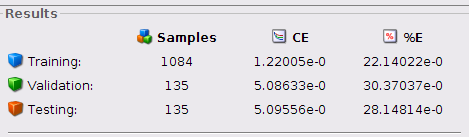
\includegraphics[width=\linewidth, keepaspectratio]{machine_learning/nn_results}
    \end{subfigure}\hfill
    \begin{subfigure}{\linewidth}
        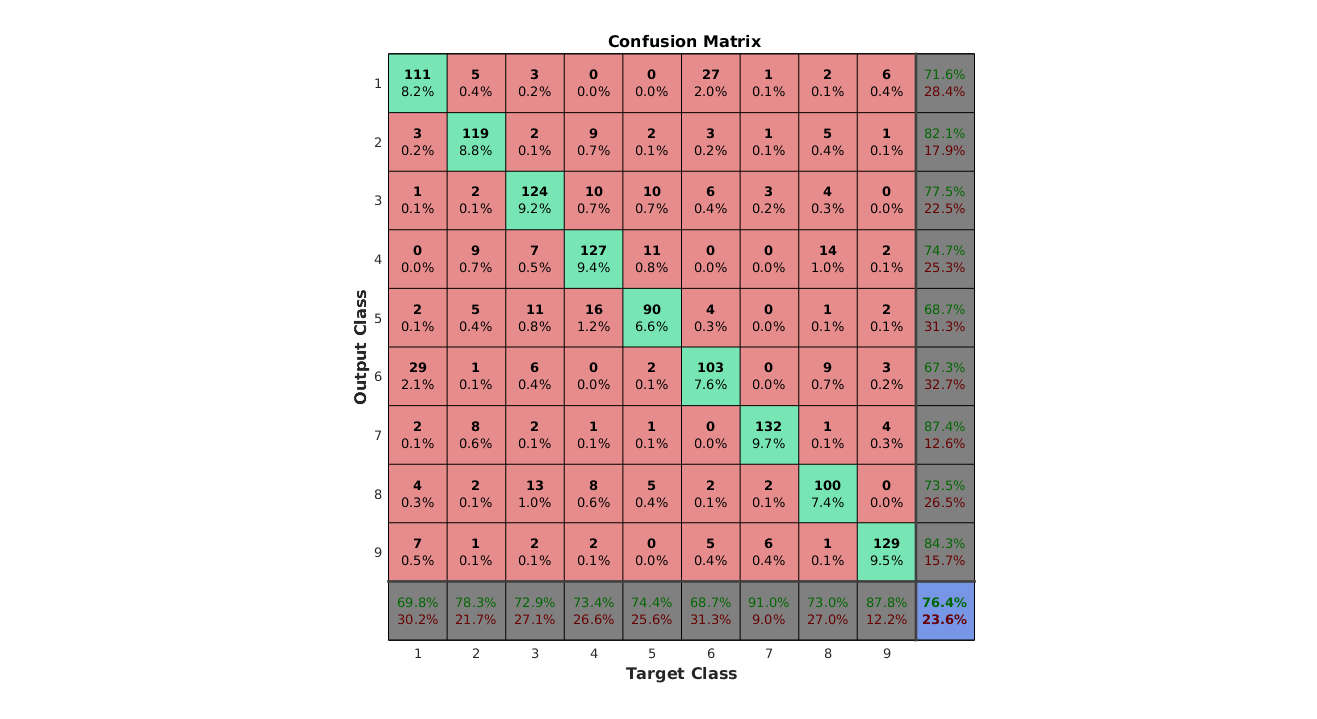
\includegraphics[width=\linewidth, keepaspectratio]{machine_learning/confusion_matrix}
    \end{subfigure}
    \caption{Αποτελέσματα Εκπαίδευσης Νευρωνικού Δικτύου. Μετρικές και Confusion Matrix.}
    \label{fig:pardo2004name-alouette}
\end{figure}